% !TEX root = collection.tex






\section{NIZK in the Hidden-Bit Model for  Graph Hamiltonian}

\begin{definition}
A Hamiltonian cycle in a graph is a cycle that visits each vertex exactly once. A Hamiltonian graph is a graph that contains a Hamiltonian cycle. More precisely, given a graph
$G=(V,E)$ with $|V|=n$, we say that $G$ is a Hamiltonian graph if there are
$x_1,\ldots,x_n\in V$ such that they are all distinct vertices, and $\forall i\in\{1,\ldots,n-1\} : (x_i,x_{i+1})\in E$,
$(x_n,x_1)\in E$.
\end{definition}


It is well known that the problem of determining if a graph is Hamiltonian is $NP$-complete.
Here we will construct a NIZK proof in the hidden-bit model (HBM) that is able to prove
that a graph is Hamiltonian.

First we define how graphs are represented as matrices.

\begin{definition}
A graph $G=(V,E)$ with $|V|=n$, can be represented as an $n\times n$ adjacency matrix $M_G$
of boolean values such that
$M_G[i,j]=\left\{
\begin{array}{l l}
1 & \text{if $(i,j)\in E$,} \\
0 & \text{otherwise.}
\end{array}
\right.$

A \emph{cycle matrix} is a matrix which corresponds to a graph that contains a Hamiltonian cycle and
contains no edges other than this cycle.

A \emph{permutation matrix} is a boolean matrix such that each row and each column has exactly one
entry equal to 1.
\end{definition}

\begin{figure}[ht]
	\centering
		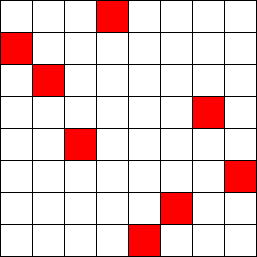
\includegraphics[height=4cm]{cycle.png}
	\caption{Cycle matrix.}
	\label{fig:cycle}
\end{figure}

\begin{figure}[ht]
	\centering
		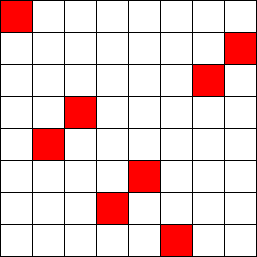
\includegraphics[height=4cm]{permutation.png}
	\caption{Permutation matrix.}
	\label{fig:permutation}
\end{figure}

Every cycle matrix is a permutation matrix, but the converse is not true.
For each size $n$, there are $n!$ different permutation matrices but
only $(n-1)!$ cycle matrices.

In Figure~\ref{fig:cycle}, one can see the cycle matrix as a cycle $(1,4,7,6,8,5,3,2)$
on the set $\{1,2,3,4,5,6,7,8\}$. In Figure~\ref{fig:permutation}, it is possible to
interpret the matrix as a permutation $(1)(2,8,6,5)(3,7,4)$ on the same set.

\begin{theorem}
There is a non-interactive zero-knowledge (NIZK) proof in the
hidden-bit model (HBM) for the problem of proving that a graph is Hamiltonian.
\end{theorem}
\proof
In the hidden-bit model (HBM), there is a random string $r$ with $\ell$ bits that the prover
can read. The prover should be able to produce a proof $\phi$ and choose a set
$I\subseteq\{1,2,\ldots,\ell\}$ such that the proof and the bits of the string corresponding to
the set $I$ will be revealed to the verifier.
\begin{table}[ht]
\centering
\begin{tabular}{r c l}
\mright{P}{\phi,I,\{r_i \mid i\in I\}}{V}
\end{tabular}
\end{table}


Let the graph be $G=(V,E)$ with $|V|=n$.
The objective is to convince the verifier that the assertion is correct (the graph $G$
is Hamiltonian).

Suppose that the random string $r$ comes from a distribution
such that this string represents the entries from an $n\times n$ cycle matrix $M_c$.
Then a proof can be produced as follows.

Since the prover $P$ knows the Hamiltonian cycle $x_1,\ldots,x_n$ in $G$, he can find a
function $\phi:V\rightarrow \{1,2,\ldots,n\}$ that puts the Hamiltonian cycle exactly
over the cycle of $M_c$. More precisely, for this function we have
$M_c[\phi(x_i),\phi(x_{i+1})]=1$ for each edge $(x_i,x_{i+1})$ in the Hamiltonian cycle of G
(we view indices modulo $n$).
This means that all the edges of $M_c$ will be covered by edges of $G$. Conversely, all the
non-edges of $G$ must be taken to non-edges of $M_c$.

So the strategy for the prover is to reveal the mapping $\phi$ and also reveal entries of $M_c$ corresponding to $\phi(e)$ where $e \notin E$. More precisely, for the set
$I=\{(\phi(u),\phi(v)) \mid (u,v)\notin E\}$, $P$ reveals
$M_c[\phi(u),\phi(v)]=0$,
which proves that $(\phi(u),\phi(v))$ is a non-edge of $M_c$.

\begin{figure}[ht]
	\centering
		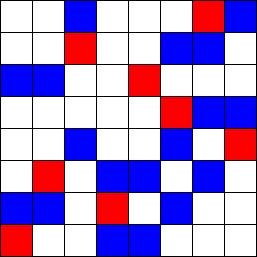
\includegraphics[height=4cm]{red_blue.png}
	\caption{Graph matrix that includes a Hamiltonian cycle. Edges are blue/red and the
                 cycle is red. White cells are non-edges.}
	\label{fig:red_blue}
\end{figure}

A visual example is shown in Figure~\ref{fig:red_blue}. The cycle graph $M_c$ given by the
random string corresponds to the red cells. These cells have value 1 in the matrix $M_c$ and
all other cells have value 0. The prover $P$ provides a bijection $\phi$ that
maps the edges of $G$ to this matrix in such a way that all red cells are covered and
some others may also be covered (blue cells). The important property guaranteed is that
all the non-edges of $G$ are mapped to cells that have a value 0 in the matrix (white cells).

This proof satisfies the three properties required for a zero knowledge proof.

\textit{Completeness:} if $P$ and $V$ are both honest, then $P$ will be able to convince
$V$ that the statement is true. That's because $P$ knows the Hamiltonian cycle of $G$,
hence he is always able to produce the mapping $\phi$.

\textit{Soundness:} if $P$ is lying and trying to prove a false statement, then he will
get caught with probability 1. If $P$ does not know any Hamiltonian cycle in $G$, then
any function $\phi$ he chooses will not cover all the edges in $M_c$. Hence there will
be an entry in the matrix $M_c$ which is one and will be revealed as a non-edge of $G$.

\textit{Zero Knowledge:} $V$ cannot get any information besides the fact that $P$
knows a Hamiltonian cycle in $G$. A simulator $S$ for this proof can be simply a machine
that generates a random permutation $\phi:V\rightarrow \{1,2,\ldots,n\}$ and reveals zeros
for all the non-edges of $\phi(G)$.

\vspace{5mm}

In this proof we assumed that the random string $r$ comes from a very specific distribution
that corresponds to cycle matrices.
Now we need to show that the general problem (where $r$ comes from a
random uniform distribution of $\ell$ bits) can be reduced into this previous scenario.

We proceed as follows.
Let the length of the random string be
$\ell=\left\lceil 3\cdot \log_2 n\right\rceil \cdot n^4$.
We view the random string $r$ as $n^4$ blocks of $\left\lceil 3\cdot \log_2 n\right\rceil$
bits and we generate a random string $r'$ of length $n^4$ such that each bit in $r'$
is 1 if and only if all the bits in the corresponding block of $r$ are equal to 1.
This way, the probability that the $i$-th bit of $r'$ equals 1 is $\Pr[r'_i=1]\approx\frac{1}{n^3}$ for every $i$.

Then we create an $n^2\times n^2$ matrix $M$ whose entries are given by the bits of $r'$.
Let $x$ be the number of one entries in the matrix $M$.
The expected value for $x$ is $\frac{n^4}{n^3}=n$.
And the probability that $x$ is exactly $n$ is noticeable. To prove that, we can use
Chebyshev's inequality:
$$\Pr[|x-n|\geq n]\leq\frac{\sigma^2}{n^2}=
\frac{n^4\cdot \frac{1}{n^3}\cdot\left(1-\frac{1}{n^3}\right)}{n^2}<\frac{1}{n}.$$
So we have $\Pr[1\leq x\leq 2n-1]>\frac{n-1}{n}$.
And the probability $\Pr[x=k]$ is maximal for $k=n$, so we conclude that
$\Pr[x=n]>\frac{n-1}{n(2n-1)}>\frac{1}{3n}$.

Now suppose that this event ($x=n$) occurred and we have exactly $n$ entries equal to 1
in matrix $M$. What is the probability that those $n$ entries are all in different rows
and are all in different columns?

We can think about the problem this way: after $k$ one entries have been added to the matrix,
the probability that a new entry will be in a different row and different column is given by
$\left(1-\frac{k}{n^2}\right)^2$. Multiplying all these values we get

\begin{align*}
\Pr[\text{no collision}] &\geq \left(1-\frac{1}{n^2}\right)^2 \cdot \left(1-\frac{2}{n^2}\right)^2
\cdots \left(1-\frac{n-1}{n^2}\right)^2 \\
& > 1 - 2\left(\frac{1}{n^2} + \frac{2}{n^2} +\cdots + \frac{n-1}{n^2}\right)
= 1 - \frac{n-1}{n} = \frac{1}{n}.
\end{align*}

Now assume that this event happened: the matrix $M$ has exactly $n$ entries equal to 1
and they are all in different rows and different columns.
Then we can define a new $n\times n$ matrix $M_c$ by selecting only those $n$ rows
and $n$ columns of $M$. By construction, $M_c$ is a permutation matrix.
The probability that $M_c$ is a cycle matrix is $\frac{(n-1)!}{n!}=\frac{1}{n}$.
An example is shown in Figures~\ref{fig:n2}~and~\ref{fig:n}.

\begin{figure}[ht]
	\centering
		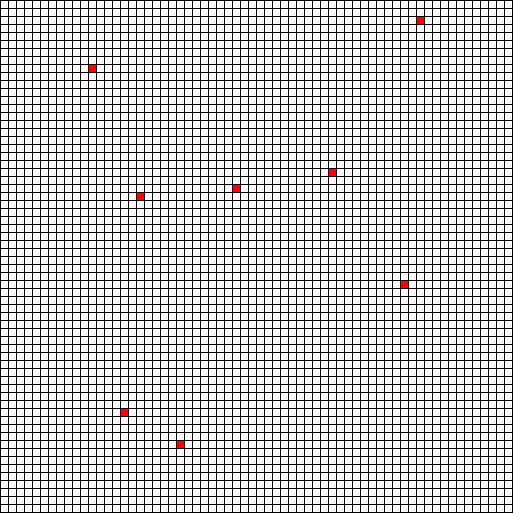
\includegraphics[height=8cm]{n2.png}
	\caption{Matrix $M$ which is $n^2\times n^2$ for $n=8$.}
	\label{fig:n2}
\end{figure}

\begin{figure}[ht]
	\centering
		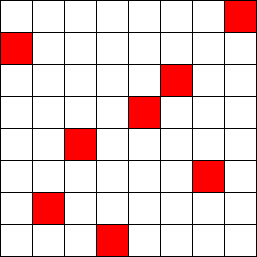
\includegraphics[height=4cm]{n.png}
	\caption{Matrix $M_c$ which is $n\times n$ for $n=8$. The construction worked,
	         because $M_c$ is a cycle matrix.}
	\label{fig:n}
\end{figure}


Now let's join all those probabilities. The probability that $M_c$ is a cycle matrix is at least
$$\frac{1}{3n}\cdot \frac{1}{n}\cdot \frac{1}{n} > \frac{1}{3n^3}.$$

If we repeat this process $n^4$ times, then the probability that $M_c$ is a cycle matrix in at least one iteration is at least
$$1-\left(1-\frac{1}{3n^3}\right)^{n^4}\approx 1-e^{-\frac{n}{3}} = 1-\mathsf{negl}(n).$$


\bigskip
The proof system works as follows. Given a random string $r$, the prover $P$ tries
to execute the construction above to obtain a cycle matrix.
If the construction fails, the prover simply reveals all the bits in the string $r$
to the verifier, who checks that the constructions indeed fails.
If the construction succeeds, the prover reveals all the entries in the random string $r$
that correspond to values in the matrix $M$ which are not used in matrix $M_c$.
The verifier will check that all these values for matrix $M$ are indeed 0.

Then the prover proceeds as in the previous scenario using matrix $M_c$: he
reveals the transformation $\phi$ and opens all the non-edges.

This process is repeated $n^4$ times. Or, equivalently, a big string of length
$\left\lceil 3\cdot \log_2 n\right\rceil \cdot n^4\cdot n^4$ is used and they are all
executed together. This produces a zero knowledge proof.

\textit{Completeness:} if $P$ knows the Hamiltonian cycle of $G$,
then he will be able to find a suitable transformation $\phi$ whenever a cycle graph is
generated by the construction.

\textit{Soundness:} if $P$ is lying and trying to prove a false statement, then he will
get caught with very high probability. If any of the $n^4$ iterations produces a cycle
graph, then $P$ will be caught. So the probability that he will be caught is
$1-e^{-\frac{n}{3}} = 1-\mathsf{negl}(n)$.

\textit{Zero Knowledge:} again $V$ cannot get any information if the construction succeeds.
And if the construction doesn't succeed, all $V$ gets is the random string $r$, which also
doesn't give any information.
\qed


\begin{theorem}
For any language $L$ in $NP$, there is a non-interactive zero-knowledge (NIZK) proof
in the hidden-bit model (HBM) for the language $L$.
\end{theorem}
\proof
The language $L^*$ of Hamiltonian graphs is $NP$-complete. So any problem in $L$ can
be reduced to a problem in $L^*$. More precisely, there is a polynomial-time function
$f$ such that
$$x\in L \Longleftrightarrow f(x)\in L^*.$$
So given an input $x$, the prover can simply calculate $f(x)$ and
produce a NIZK proof in the hidden-bit model for the fact that $f(x)\in L^*$.
Then the verifier just needs to calculate $f(x)$ and check if the proof for the fact
$f(x)\in L^*$ is correct.
\qed

\begin{theorem}\label{the:NIZK_NP}
For any language $L$ in $NP$, there is a non-interactive zero-knowledge (NIZK) proof
in the common reference string (CRS) model for the language $L$.
\end{theorem}
\proof
In Theorem~\ref{thm:NIZK-amplify} it was shown that any NIZK proof in the hidden-bit model can
be converted into a NIZK proof in the standard (common reference string) model by using
a trapdoor permutation.
\qed

\section*{Exercises}
\begin{exercise}
\textbf{Multi-statement NIZK.} The NIZK proof system we constructed in class required a fresh common random string (CRS) for each statement proved. In various settings we would like to reuse the same random string to prove multiple theorem statements while still preserving the zero-knowledge property.
    
    A multi-statement NIZK proof system $(K,P,V)$ for a language $L$ with corresponding relation $R$ is a NIZK proof system for $L$ with a stronger zero-knowledge property, defined as follows: $\exists$ a PPT machine $\mathcal{S} = (\mathcal{S}_1,\mathcal{S}_2)$ such that $\forall$ PPT machines $A_1$ and $A_2$ we have that:
    \[\left|\Pr\left[\begin{split}\sigma \gets K(1^\kappa),\\ (\{x_i,w_i\}_{i \in [q]},\textsf{state}) \gets A_1(\sigma),\\ \text{ such that } \forall i \in [q], (x_i,w_i)\in R\\\forall i \in [q],  \pi_i \gets P(\sigma, x_i,w_i);\\
    A_2(\textsf{state}, \{\pi_i\}_{i \in [q]}) =1\end{split}\right]
    -
    \Pr\left[\begin{split}(\sigma,\tau) \gets \mathcal{S}_1(1^\kappa),\\ (\{x_i,w_i\}_{i \in [q]},\textsf{state}) \gets A_1(\sigma),\\\text{ such that } \forall i \in [q], (x_i,w_i)\in R\\\forall i \in [q],  \pi_i \gets \mathcal{S}_2(\sigma, x_i,\tau);\\ A_2(\textsf{state}, \{\pi_i\}_{i \in [q]})=1\end{split}\right]\right|
    \leq \textsf{negl}(\kappa).
    \]
    
    Assuming that a single statement NIZK proof system $(K,P,V)$ for NP exists, construct a multi-statement NIZK proof system $(K',P',V')$ for NP.\\
\textbf{Hint:} Let $g: \{0,1\}^\kappa \rightarrow \{0,1\}^{2\kappa}$ be a length doubling PRG. Let $K'$ output the output of $K$ along with $y$, a random $2\kappa$ bit string. To prove $x \in L$ the prover $P'$ proves that $\exists (w,s)$ such that either $(x,w)\in R$ or $y = g(s)$.
\end{exercise}
